\documentclass[12pt]{article}
\usepackage[top=1in,left=1in, right = 1in, footskip=1in]{geometry}

\title{Avidity and immunogenicity}
\usepackage{graphics}
\usepackage{adjustbox}

\newcommand{\eref}[1]{(\ref{eq:#1})}
\newcommand{\fref}[1]{Fig.~\ref{fig:#1}}
\newcommand{\Fref}[1]{Fig.~\ref{fig:#1}}
\newcommand{\sref}[1]{Sec.~\ref{#1}}
\newcommand{\frange}[2]{Fig.~\ref{fig:#1}--\ref{fig:#2}}
\newcommand{\tref}[1]{Table~\ref{tab:#1}}
\newcommand{\tlab}[1]{\label{tab:#1}}

\usepackage{amsthm}
\usepackage{amsmath}
\usepackage{amssymb}
\usepackage{amsfonts}

\usepackage{hyperref}
\usepackage{natbib}
\usepackage{hyperref}
\bibliographystyle{chicago}
\date{\today}

\usepackage{xspace}
\newcommand*{\ie}{i.e.\@\xspace}

\usepackage{color}

\newcommand{\Rx}[1]{\ensuremath{{\mathcal R}_{#1}}} 
\newcommand{\Ro}{\Rx{0}}
\newcommand{\RR}{\ensuremath{{\mathcal R}}}
\newcommand{\tsub}[2]{#1_{{\textrm{\tiny #2}}}}
\newcommand{\tsup}[2]{#1^{{\textrm{\tiny #2}}}}


\newcommand{\comment}[3]{\textcolor{#1}{\textbf{[#2: }\textsl{#3}\textbf{]}}}
\newcommand{\jd}[1]{\comment{cyan}{JD}{#1}}
\newcommand{\swp}[1]{\comment{magenta}{SWP}{#1}}
\newcommand{\hotcomment}[1]{\comment{red}{HOT}{#1}}

\begin{document}
\maketitle

Let $H^{ij}$ denote a titer value from hemagglutination-inhibition (HI) assays of virus isolate $i$ against antisera $j$.
We can decompose this titer value to make inference about non-antigenic variables \citep{li2013single}:
\begin{equation}\label{eq:decomp}
H^{ij} = J^i K^{ij} A^j,
\end{equation}
where $J^i$ is the effect of virus, $A^j$ is the effect of antisera, and $K^{ij}$ is the affinity antibody $j$ to virus $i$.
We expect $J^i$ to be inversely correlated with virus avidity, the ability of virus to bind to cellular receptor: strains with higher binding avidity will be able to bind to red blood cells even at higher antibody concentration (i.e., lower HI titer) \citep{ndifon2011new}.
$A^j$ is the effect of antisera and represents the concentration of antibodies.
We expect $A^j$ to be positively correlated with immunogenecity: virus strains that are more immunogenic will induce higher antibody concentration in antiserum $j$, requiring higher dilution.
Hereafter, $H^{ij}$, $J^i$, $K^{ij}$, and $A^j$ refer to $\log_2$-transformed values of the corresponding quantities so that titers can be represented as a sum:
\begin{equation}
H^{ij} = J^i + K^{ij} + A^j. 
\end{equation}

\cite{bedford2014integrating} suggested that the estimate of HI titer can be written as 
\begin{equation}
\hat{H}^{ij} = \frac{J^i + A^j}{2} - d(i, j)
\end{equation}
where $J^i$ and $A^j$ are assumed to come from normal distributions with mean and variance defined as empirical mean and variance meaximum $\log_2$ HI titer across virus and antiserum, respectively; $d(ij)$ represents Euclidean distance between virus $i$ and antiserum $j$.
Dividing the sum of $J^i$ and $A^j$ by 2 accounts for the fact that mean $\log_2$ maximum HI titers are counted twice but effectively reduces variance of ``true'' $J^i$ and $A^j$ by a factor of 4.
Instead, we can write 
\begin{equation}
\hat{H}^{ij} = \beta_0 + J^i + A^j - d(i, j)
\end{equation}
where $J^i$ and $A^j$ now have a mean of 0. This formulation better reflects Equation~\ref{eq:decomp} and allows us to translate $\beta_0 - d(i, j)$ as $K^{ij}$.
I've also incorporated censored likelihood for HI titers, following \cite{bedford2014integrating}.

\section{Empirical Bayesian}

First, we begin with empirical Baeysian assumptions.
Variance of $J^i$ and $A^j$ follow empirical variance of maximum titer across virus and antiserum, respectively.
Likewise, $\beta_0$ is given a point prior of average of empirical mean maximum titers across virus and antiserum (this is same as $E[(J^i + A^j)/2]$ from Equation~3).

\begin{figure}
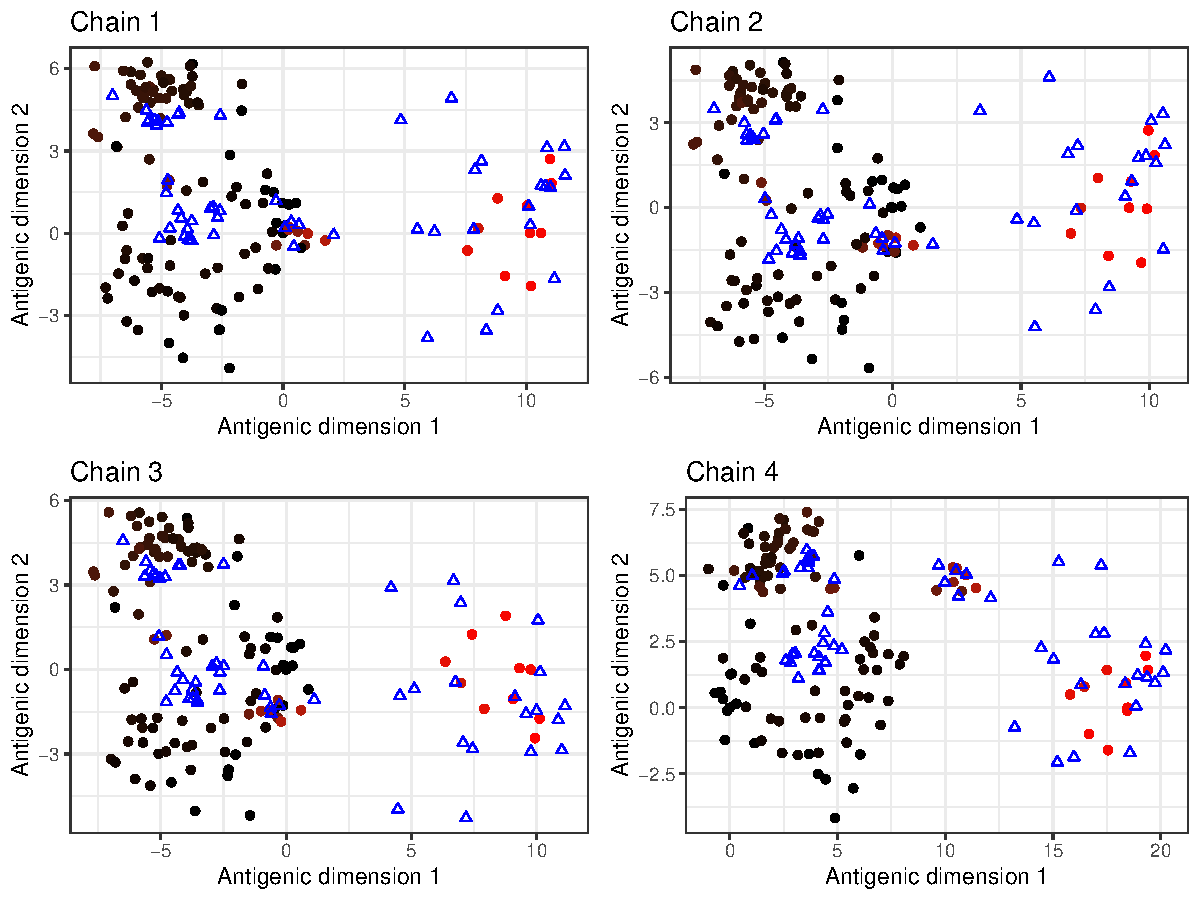
\includegraphics[width=\textwidth]{../figure/h1n1_map.pdf}
\caption{Median positions of virus. 
Blue triangles represent positions of antiserum.
Circles represent positions of virus.
}
\end{figure}

For exploratory purposes, I ran foure chains for 4000 iterations.
All four chains ran without any error but it seems like there are local minimas.
First three chains converged to different locations in antigenic space from the last chain (Figure~1). 
In chain 4, we have a separate cluster in the middle but that cluster is not observed in other chains. 

We might think that these chains did not converge. 
Indeed, when we look at Gelman-Rubin Rhat values on virus and serum positions, they go as high as 2.2.
Howeve, Gelman-Rubin statistics for all other parameters (i.e., effect of virus, effect of serum, and log-posterior density), they all stay below 1.03. 
This suggests that we can robustly estimate $J^i$ and $A^j$ but not the virus or serum positions;
informing the positions with phylogeny might help us better identify their positions.

\begin{figure}
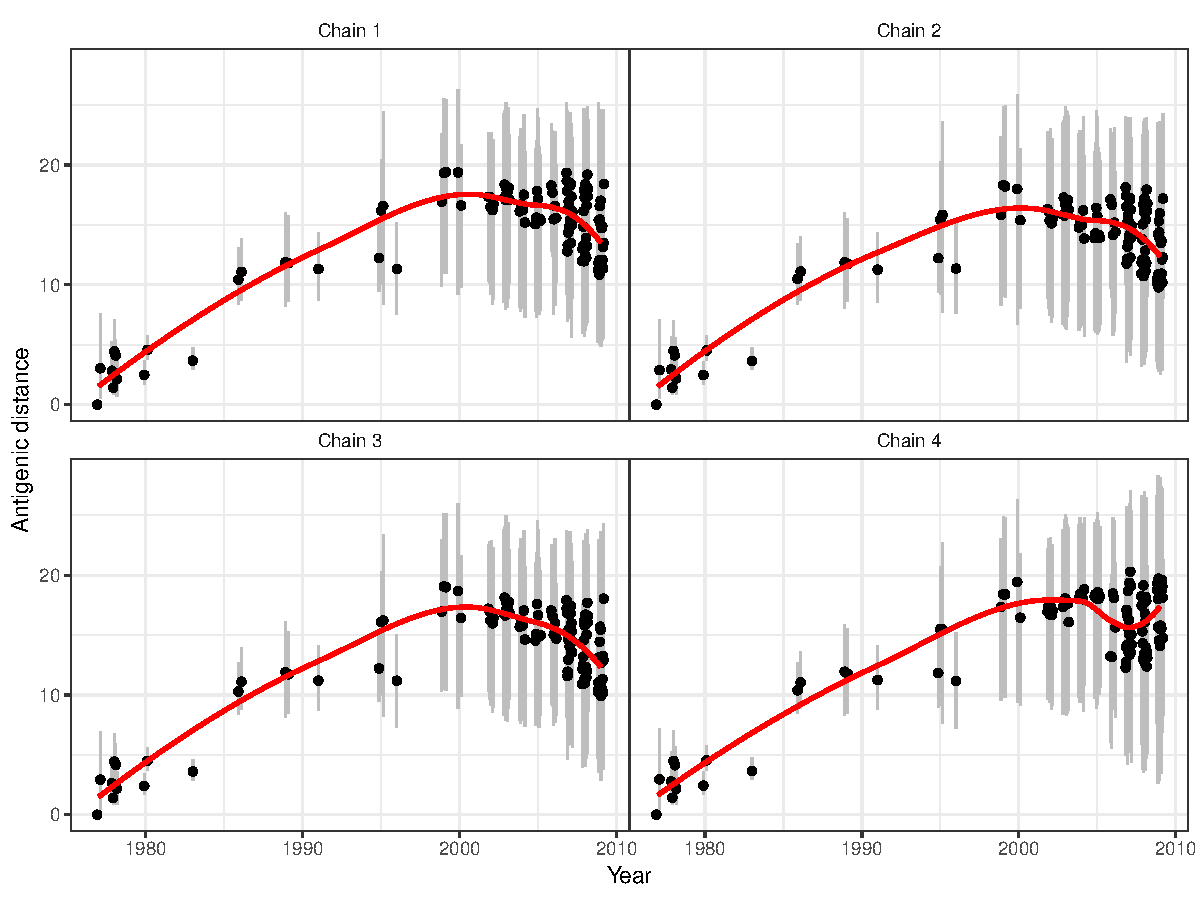
\includegraphics[width=\textwidth]{../figure/h1n1_distance.pdf}
\caption{
Antigenic distance over time.
}
\end{figure}

How does antigenic distance change over time? Is this something we can estimate robustly?
We can compare antigenic distance relative to A/USSR/90/1977 strain (Figure~2).
It turns out that difference in antigenic distance over time is also fairly robust.
Chain 4 shows a slightly different behaviour after 2001 but the general patterns are not too different.

\begin{figure}
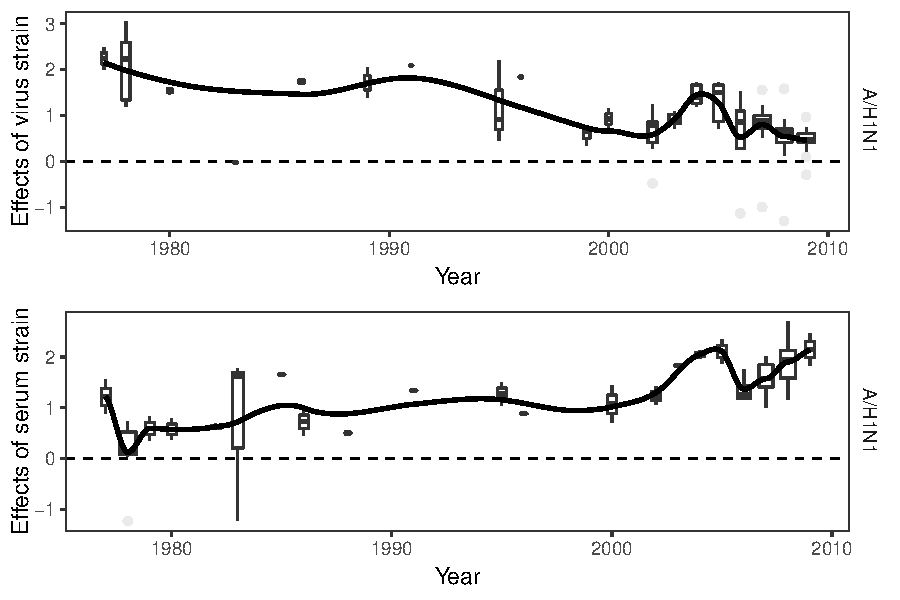
\includegraphics[width=\textwidth]{../figure/h1n1_effect.pdf}
\caption{Boxplots of median effects of virus and serum.}
\end{figure}

We can also look at how estimates of virus effect and serum effect changes over time (Figure~3).
This is something we know that we can estimate robustly, based on the Gelman-Rubin statistics.
We can make two conclusions from this.
First, there is gradual decrease in the effect of virus ($J^i$) and gradual increase in the effect of serum ($A^j$) over time. This could be interpreted as increase in virus avidity and immunogenecity towards 2009 pandemic? 
It also seems like something might have happened in 2004-2005 (sudden change in both $J^i$ and $A^j$).
Second, the fact that medians of $J^i$ and $A^j$ are greater than zero suggests that the point prior we imposed on $\beta_0$ is inappropriate.

\begin{figure}
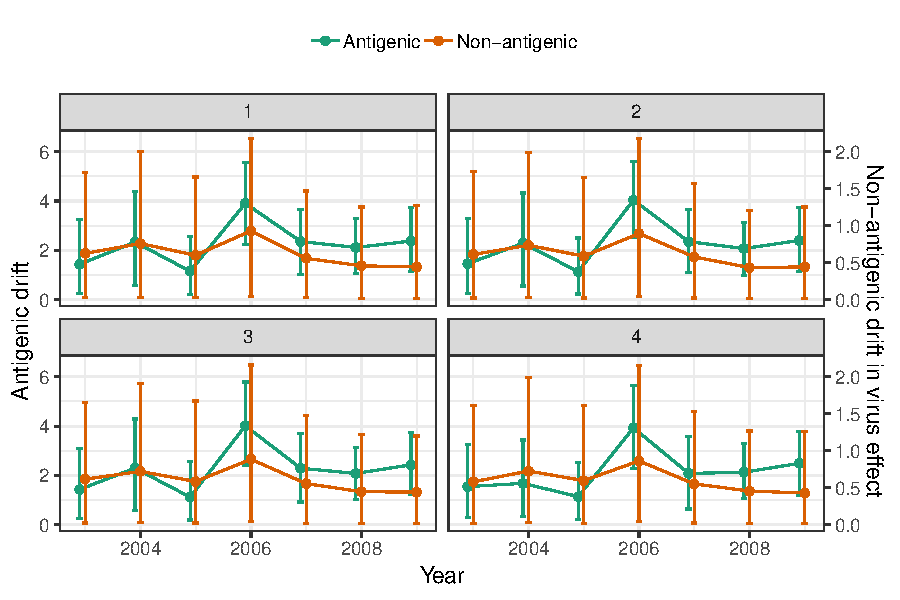
\includegraphics[width=\textwidth]{../figure/h1n1_drift.pdf}
\caption{Comparing antigenic and non-antigenic drift.}
\end{figure}

Can we consider the hypothesis by \citep{hensley2009hemagglutinin}?
The idea is that virus avidity drives antigenic evolution.
We can define antigenic drift as distance between mean locations in consecutive years.
Similarly, we can define non-antigenic drift as absolute difference in mean virus effect ($J^i$) in consecutive years.
We can do this over posterior samples and plot them into a single figure (Figure~4).
We do this from 2002 to 2009 because those are the years where we have data for consecutive years.
It seems likde these ``drift'' can be estimated fairly robustly, even though we have local minima problems.

Surprisingly, we see similarity in patterns of antigenic drift and non-antigenic drift (Figure~4).
However, correlation between antigenic and non-antigenic drift across posterior is rather unclear: 0.2 (95\% CI: -0.69 - 0.86).

\section{Relaxing Empirical Bayesian}

\begin{figure}
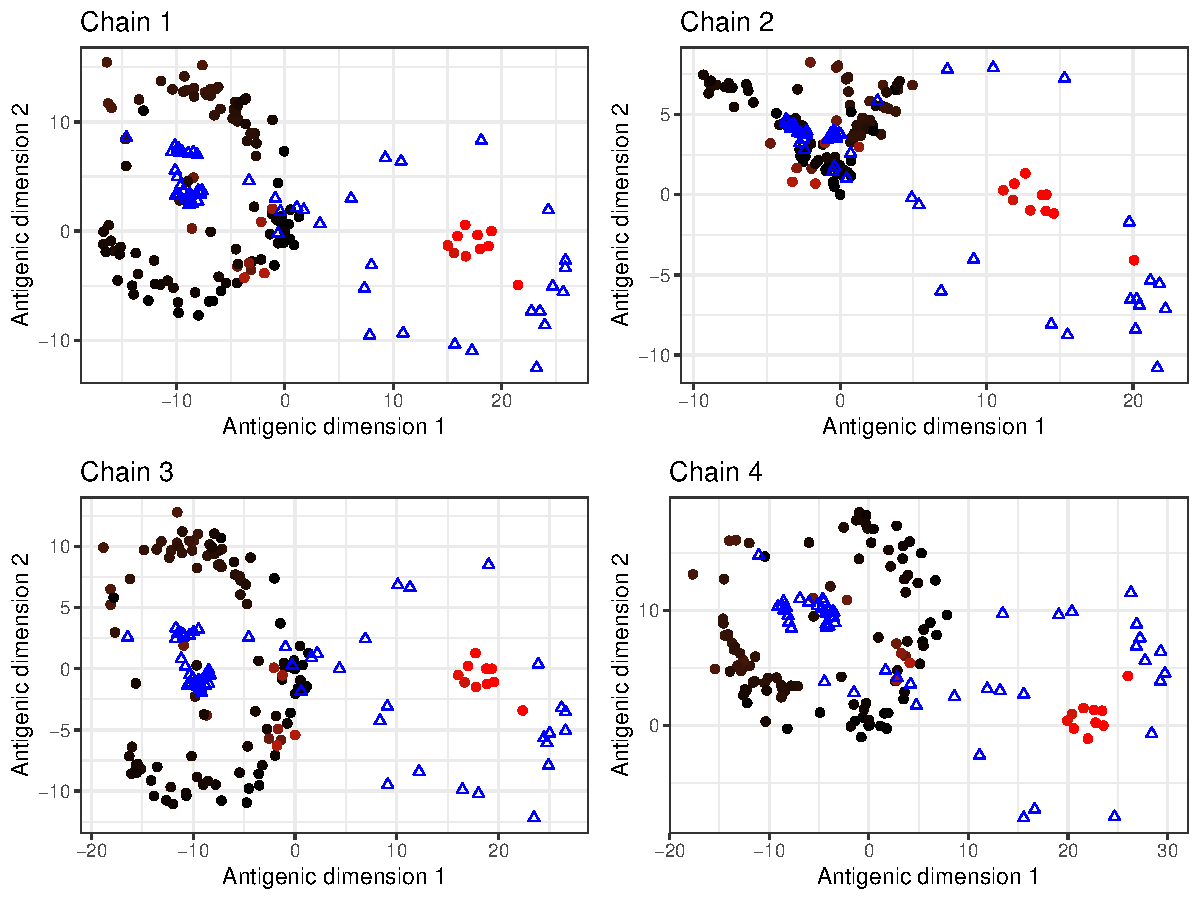
\includegraphics[width=\textwidth]{../figure/h1n1_map_relax.pdf}
\caption{Median positions of virus. 
Blue triangles represent positions of antiserum.
Circles represent positions of virus. Color gradient from red to black represents change in time.
}
\end{figure}

I relax the empirical Bayesian assumption. Previously, $\beta_0$ was given a point prior of approximately 10. Instead, I assume that $\beta_0$ is normally distributed with standard deviation of 1.
This time, I found three posterior modes (Figure~5). Their log-posterior densities are similar so I think we can treat them as true posterior modes. 
Besides serum location and virus location, all other parameters are well-mixed (with Gelman-Rubin statistic less than 1.1).

There are two robust features we can infer from three maps. 
First, there is a clear clustering of viruses before 1985 and after 1985. 
Second, there is a virus strain that appears to be different from the rest of the 1977-1985 cluster.

\begin{figure}
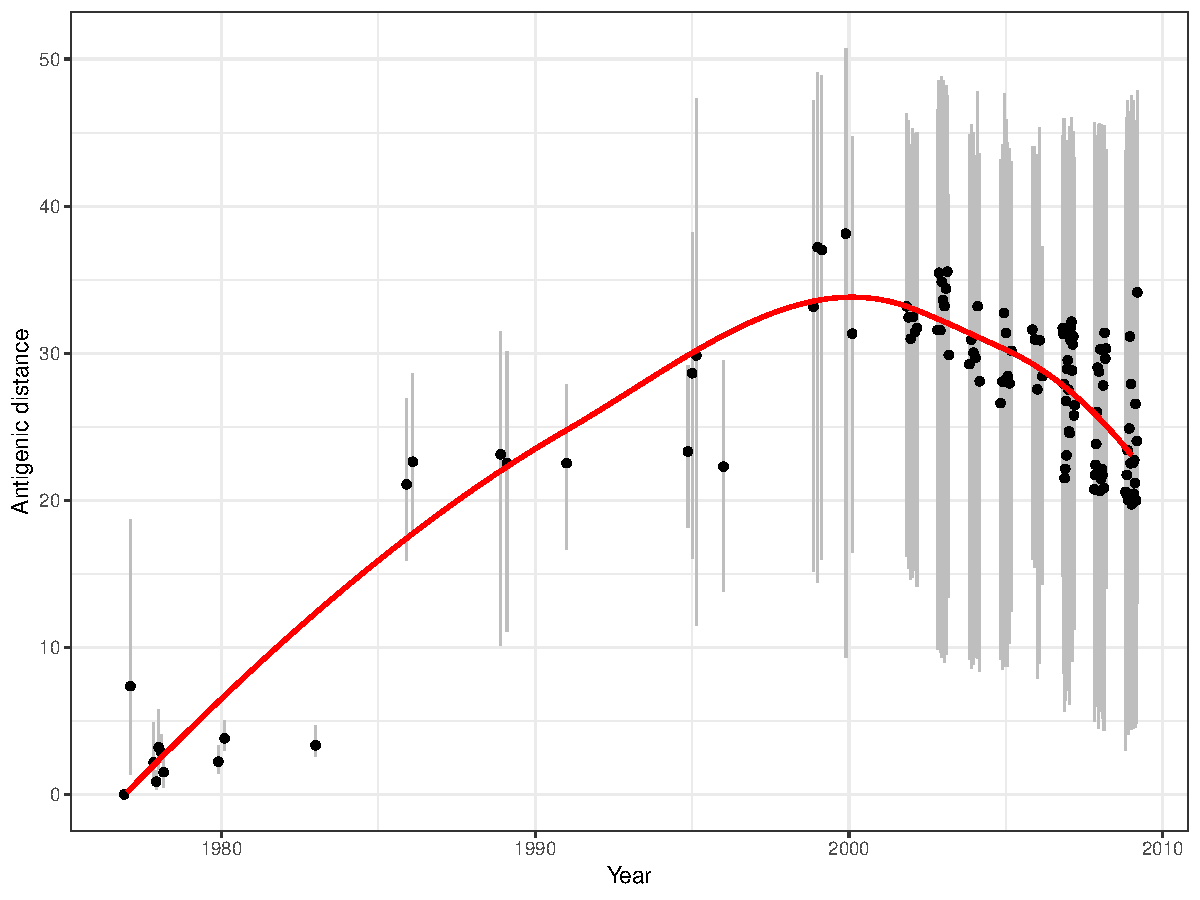
\includegraphics[width=\textwidth]{../figure/h1n1_distance_relax.pdf}
\caption{
Antigenic distance over time.
}
\end{figure}

When we look at how antigenic distance changes over time, this observation becomes clearer (Figure~6).
It seems like  A/USSR/92/1977 is different from other virus strains from 1977-1985.
Moreover, we find a quadratic pattern in antigenic distance over time.
If we had forced an increasing direction in one dimension, we would not have been able to see this pattern.

Another important point we can make is that relaxing the assumption on $\beta_0$ increased Euclidean distance bewteen viruses by almost two fold. 
It's also surprising to note that the posterior for $\beta_0$ has a mean of approximately 18 and standard deviationof 0.7, even though we had a reasonably tight prior around 10. 
It's slightly worrying because these observations show that our inference may depend heavily on our prior assumptions.
We may want to constrain the map a little more by imposing hierarchical prior in the Euclidean map (homologous virus and antiserum are assigned same prior mean location). Then, phylogeny will constrain these mean locations, rather than the actual locations of virus and antiserum.


\begin{figure}
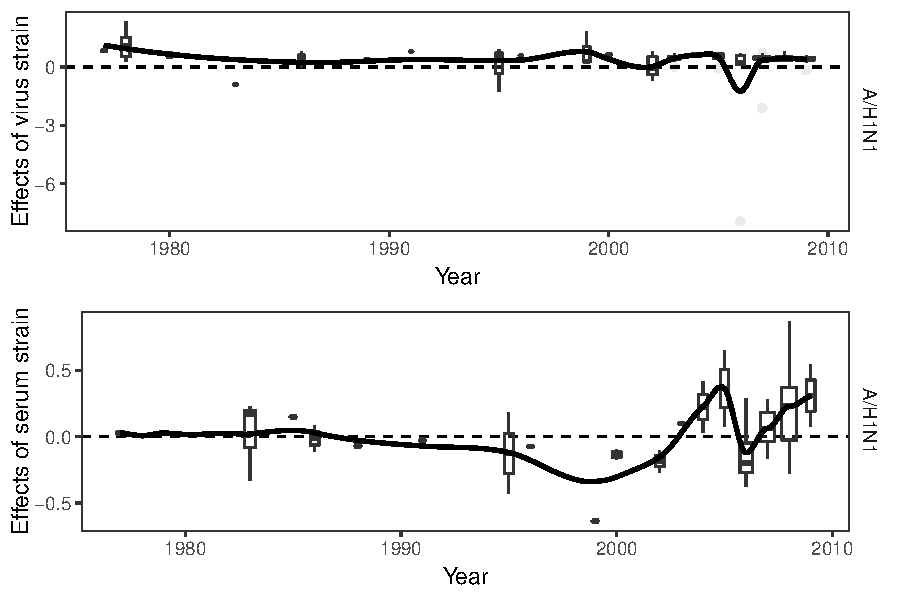
\includegraphics[width=\textwidth]{../figure/h1n1_effect_relax.pdf}
\caption{Boxplots of median effects of virus and serum.}
\end{figure}

Finally, temporal patterns in non-antigenic variables and immunogenecity change when we relax our assumptions on $\beta_0$.
We no longer observe long-term trends... but we can still a different pattern in 2005, as predicted before.
However, we can now see that the sudden change in the smooth line in the non-antigenic varaible plot in year 2005 is driven by a single virus, which is A/SolomonIslands/3/2006.
Based on a quick google search, all I can find is that A/SolomonIslands/3/2006 was recommended by WHO for vaccines in 2007-2008 for northern hemisphere and 20008 for southern hemisphere.

Still a lot more to think about ...

(This list has not been updated) Things to do and think about:
\begin{itemize}
	\item Think about what these local minimas mean?
	\item Analyze other influenze subtypes
	\item Include phylogeny? See \cite{bedford2014integrating}. I think phylogeny can inform location of virus as well as $J^i$ and $A^j$?
	\item Can we associate $J^i$ and $A^j$ with other quantities (e.g., number of positive cases)
	\item Can we get more recent titer data? ``Reports prepared for the WHO annual consultation on the composition of influenza vaccine'' include titer tables in pdf files but it's not clear how I can get them
\end{itemize}



\bibliography{bayes}

\end{document}
